\documentclass{article}

% if you need to pass options to natbib, use, e.g.:
% \PassOptionsToPackage{numbers, compress}{natbib}
% before loading nips_2017
%
% to avoid loading the natbib package, add option nonatbib:
% \usepackage[nonatbib]{nips_2017}

\usepackage[final]{nips_2017}

% to compile a camera-ready version, add the [final] option, e.g.:
% \usepackage[final]{nips_2017}

\usepackage[utf8]{inputenc} % allow utf-8 input
\usepackage[T1]{fontenc}    % use 8-bit T1 fonts
\usepackage{hyperref}       % hyperlinks
\usepackage{url}            % simple URL typesetting
\usepackage{booktabs}       % professional-quality tables
\usepackage{amsfonts}       % blackboard math symbols
\usepackage{nicefrac}       % compact symbols for 1/2, etc.
\usepackage{microtype}      % microtypography
\usepackage{float}
\usepackage{graphicx}
\usepackage{changepage}

\title{Wybrane zagadnienia sztucznej inteligencji - Sprawozdanie 3 - Uczenie ze wzmocnieniem i nadzorowane w grach}

% The \author macro works with any number of authors. There are two
% commands used to separate the names and addresses of multiple
% authors: \And and \AND.
%
% Using \And between authors leaves it to LaTeX to determine where to
% break the lines. Using \AND forces a line break at that point. So,
% if LaTeX puts 3 of 4 authors names on the first line, and the last
% on the second line, try using \AND instead of \And before the third
% author name.

\author{Tomasz Pastusiak \And{Leszek Kawecki}}

\begin{document}
% \nipsfinalcopy is no longer used

\maketitle


\section{Badanie Q-learningu}

\begin{figure}[H]
  \centering
  \fbox{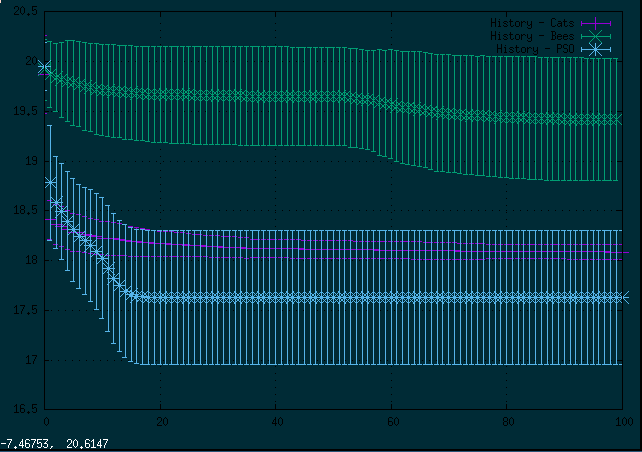
\includegraphics[width=0.9\textwidth]{img/ackley_10_100.png}}
  \caption{Test image}
  \label{fig:ackley_10_100}
\end{figure}

\section{Badanie uczenia nadzorowanego}

\subsection{Badanie dla sieci neuronowej}

\subsubsection{Wpływ rozmiaru zbioru uczącego na wyniki}

\begin{center}
  \begin{tabular}{ | l | l | l | l | }
    \hline
    liczba gier w zbiorze & próba 1 & próba 2 & próba 3 \\ \hline
    2 & (W:450, D:133, L:417) & (W:415, D:148, L:437) & (W:454, D:134, L:412) \\ \hline
    10 & (W:438, D:129, L:433) & (W:483, D:168, L:349) & (W:450, D:107, L:443) \\ \hline
    100 & (W:653, D:58, L:289) & (W:495, D:125, L:380) & (W:442, D:183, L:375) \\ \hline
    500 & (W:652, D:134, L:214) & (W:753, D:118, L:129) & (W:718, D:76, L:206) \\ \hline
    1000 & (W:676, D:178, L:146) & (W:431, D:154, L:415) & (W:841, D:78, L:81) \\ \hline
    5000 & (W:869, D:86, L:45) & (W:848, D:114, L:38) & (W:913, D:54, L:33) \\ \hline
    10000 & (W:914, D:50, L:36) & (W:865, D:110, L:25) & (W:907, D:55, L:38) \\ \hline
  \end{tabular}
\end{center}


\section{Porównanie Q-learningu i uczenia nadzorowanego}



\end{document}

